\chapter{UART Block}
\label{ch:rs232}
RS232 modul er hardware implemeteret med SM,  dataforbindelse mellem SM og KI anvender en RS232-protokol, dette betyder at UART signalet fra SM skal level konverteres til RS232-protokol. 
\section{Overordnet design}
Nedenfor vises det overordnet blokdiagram for RS232 modul, samt beskrivelser af de enkel blokke.
\begin{figure}[H]
\centering
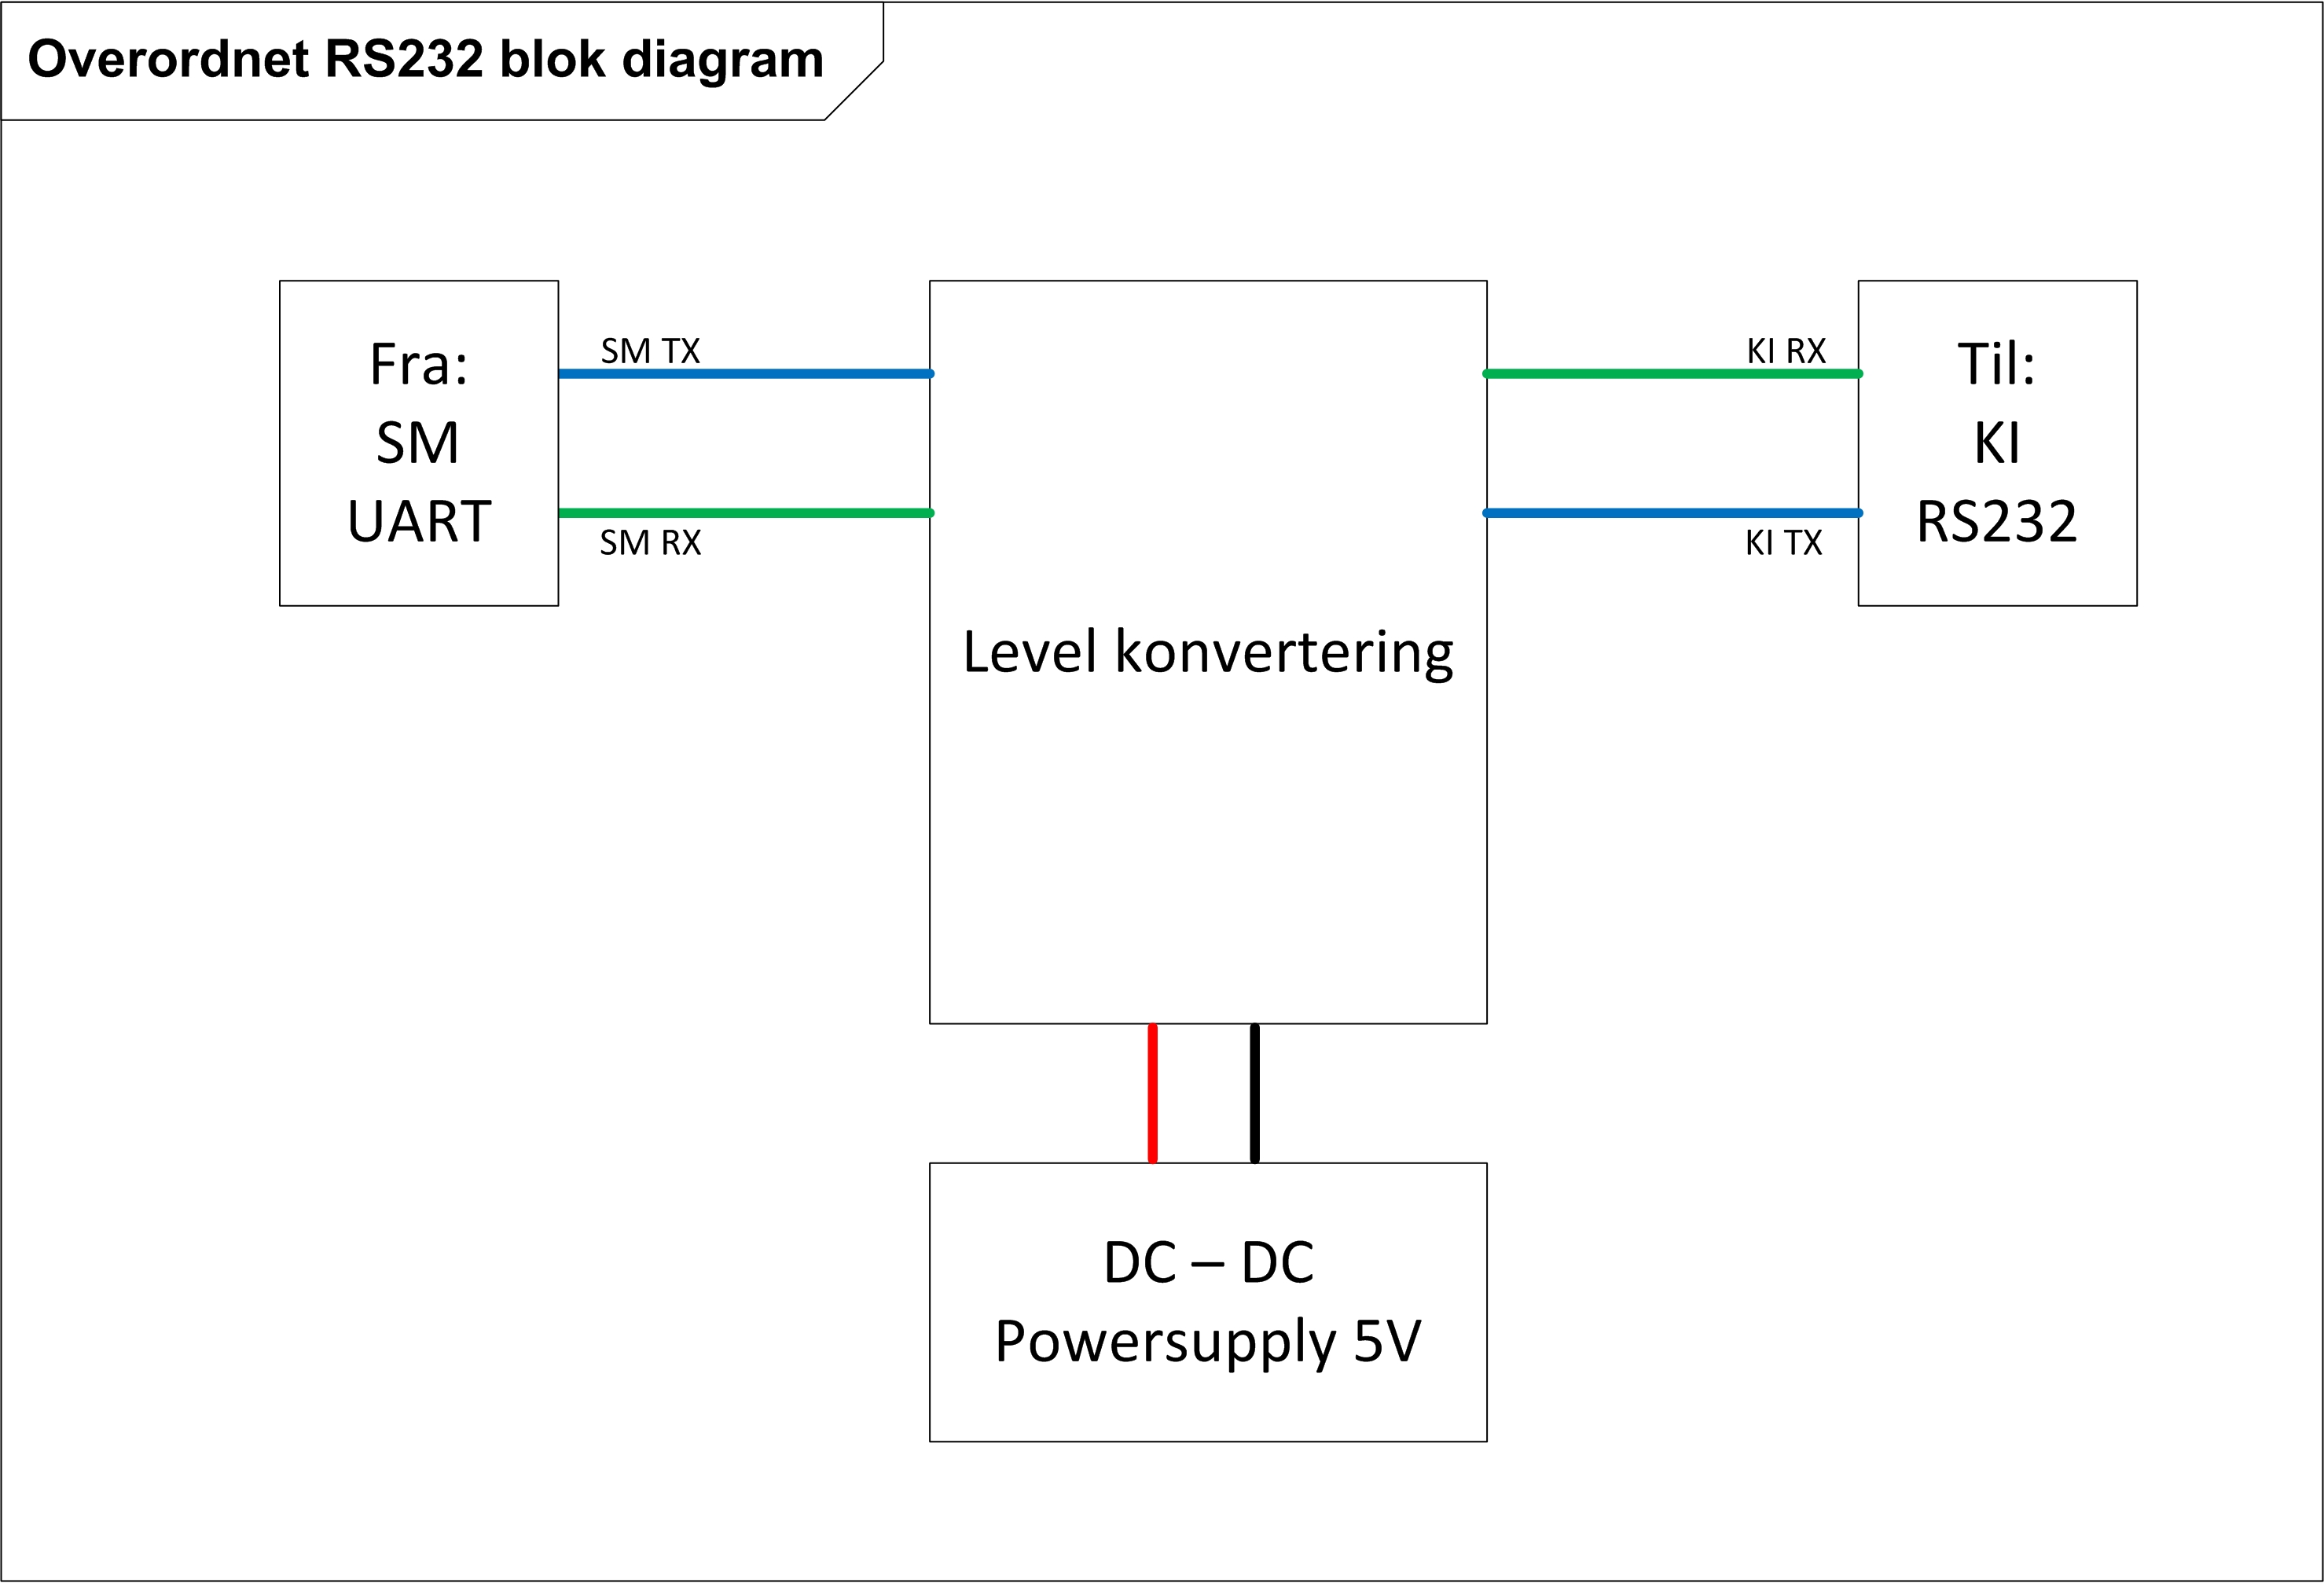
\includegraphics[scale=1]{billeder/RS232ModulBlok}
\caption{Blokdiagram for UART Block}
\label{fig:RS232ModulBlok}
\end{figure}
\newpage
\subsection{Blokke}
Nedenfor beskrives de enkelte blokke illustreret på \textit{Figur~\ref{fig:RS232ModulBlok}}
\subsubsection{SM UART}
Se SM, overordnet design.
\subsubsection{Indikator TX}
Indikere om der sendes data.
\subsubsection{Indikator RX}
Indikere om der modtages data.
\subsubsection{Level konverter}
Level konverter signalet fra SM UART til RS232-protokol.
\subsubsection{konnektor RS232}
DB9 stik der forbindes med kabel til KI.
\subsubsection{DC - DC PowerSupply 5V}
Se powersuply afsnittet.
\newpage
\section{Nedbrydning af blokke}
For at gøre designet af de forskellige blokke mere overskuelig nedbrydes de enkle blokke fra det overordnede blokdiagram.
\subsection{SM UART}
Se SM, nedbrydning af design.
\subsection{Indikator TX}
Indikator TX viser med en diode om der transmittes data fra SM.
\begin{figure}[H]
\centering
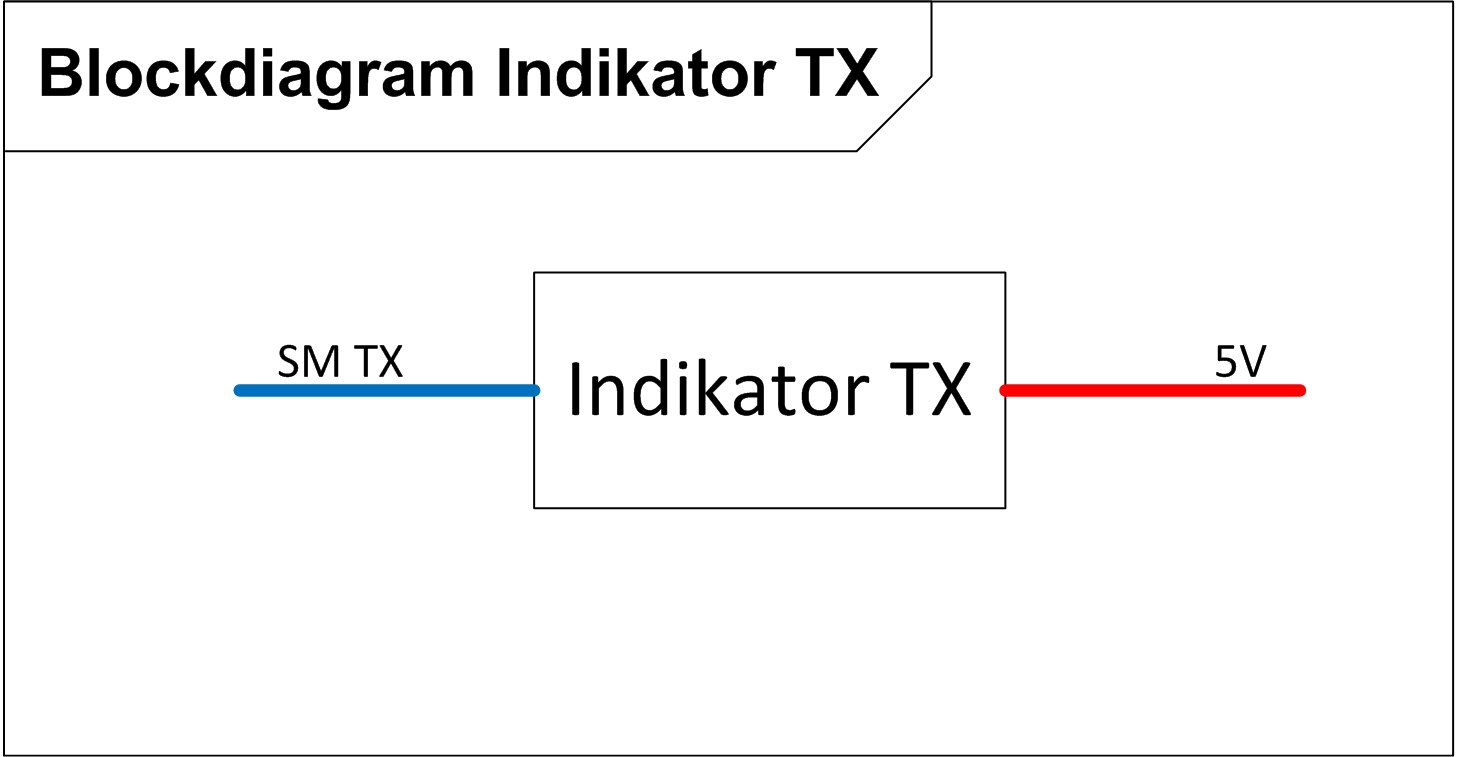
\includegraphics[scale=1]{billeder/Indikator_TXblok}
\caption{Blokdiagram for Indikator TX}
\label{fig:Indikator_TX}
\end{figure}
\subsubsection{Signalbeskrivelser:}
For signalbeskrivelser se \textit{tabel~\ref{table:Indikator_TX}}
\begin{table}[H]
\begin{tabular}{|p{3cm}|p{3cm}|p{3cm}|p{4.5cm}|} \hline
\cellcolor[gray]{0.85}Signal navn& \cellcolor[gray]{0.85}Type &\cellcolor[gray]{0.85}Spænding&\cellcolor[gray]{0.85}Beskrivelse\\ \hline
SM TX & Analog & $\sim$0V til $\sim$5V & TX fra PSoC blokken.\\ \hline
5V & Analog & 5V$\pm$0.2V & 5V forsyning der leveres fra powersupplyen beskrevet under powersupply. \\ \hline
\end{tabular}
\caption{Tabel over signaler i Indikatoren TX blokken}
\label{table:Indikator_TX}
\end{table}
\newpage
\subsection{Indikator RX}
Indikator RX viser med en diode om der modtages data fra SM.
\begin{figure}[H]
\centering
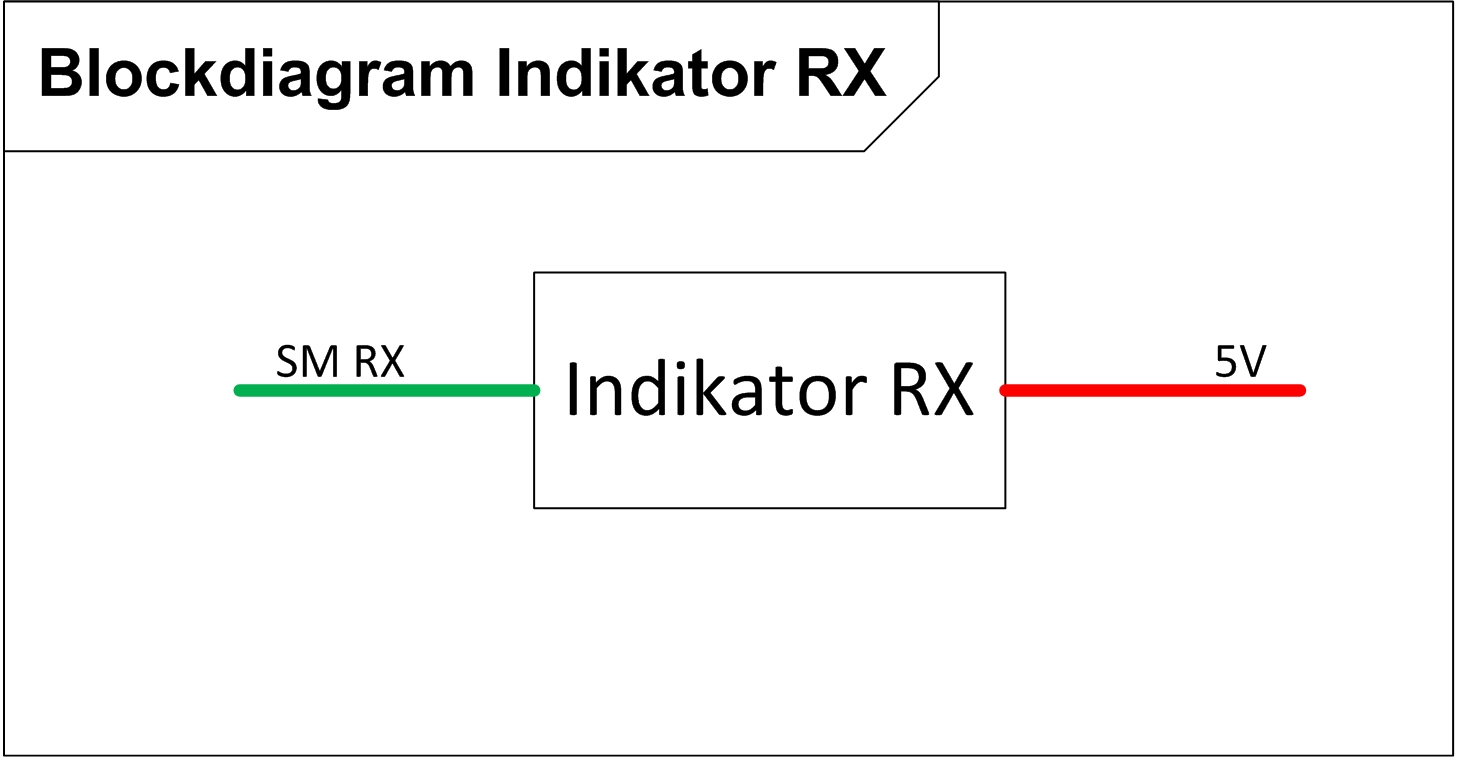
\includegraphics[scale=1]{billeder/Indikator_RXblok}
\caption{Blokdiagram for Indikator RX}
\label{fig:Indikator_RX}
\end{figure}
\subsubsection{Signalbeskrivelser:}
For signalbeskrivelser se \textit{tabel~\ref{table:Indikator_RX}}
\begin{table}[H]
\begin{tabular}{|p{3cm}|p{3cm}|p{3cm}|p{4.5cm}|} \hline
\cellcolor[gray]{0.85}Signal navn& \cellcolor[gray]{0.85}Type &\cellcolor[gray]{0.85}Spænding&\cellcolor[gray]{0.85}Beskrivelse\\ \hline
SM RX & Analog & $\sim$0V til $\sim$5V & TR fra PSoC blokken.\\ \hline
5V & Analog & 5V$\pm$0.2V & 5V forsyning der leveres fra powersupplyen beskrevet under powersupply. \\ \hline
\end{tabular}
\caption{Tabel over signaler i Indikator RX blokken}
\label{table:Indikator_RX}
\end{table}
\newpage
\subsection{Level konverter}
Level konverter signalet fra SM UART til RS232-protokol.
\begin{figure}[H]
\centering
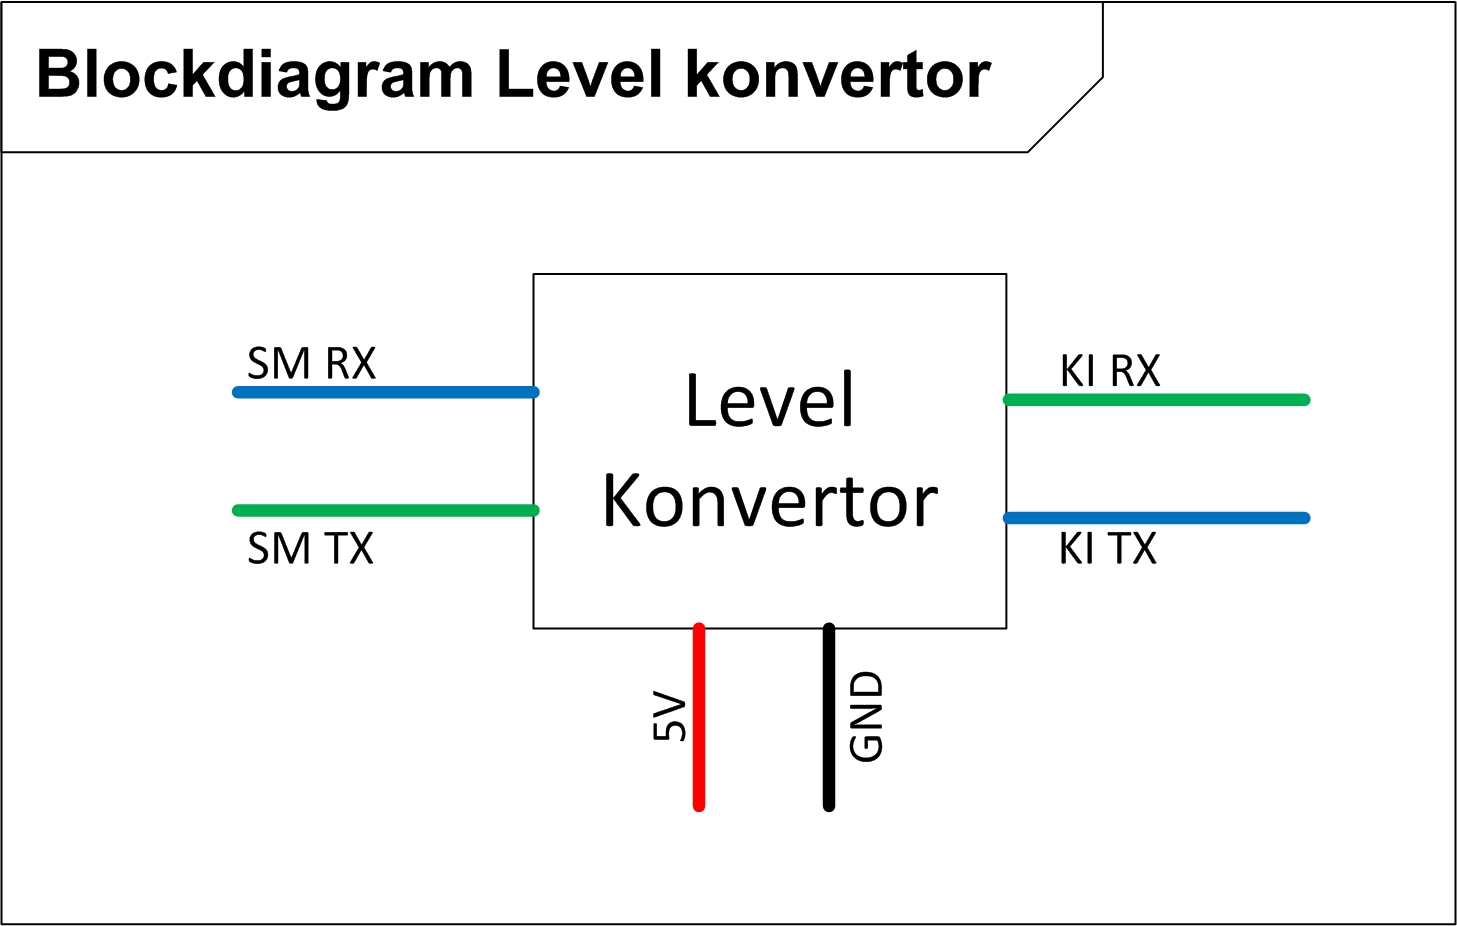
\includegraphics[scale=1]{billeder/Level_konverter}
\caption{Blokdiagram for level konverter}
\label{fig:LevelKonverter}
\end{figure}
\subsubsection{Signalbeskrivelser:}
For signalbeskrivelser se \textit{tabel~\ref{table:SignalerLevelKonverter}}
\begin{table}[H]
\begin{tabular}{|p{3cm}|p{3cm}|p{3cm}|p{4.5cm}|} \hline
\cellcolor[gray]{0.85}Signal navn& \cellcolor[gray]{0.85}Type &\cellcolor[gray]{0.85}Spænding&\cellcolor[gray]{0.85}Beskrivelse\\ \hline
SM TX & Analog & $\sim$0V til $\sim$5V & TX fra PSoC blokken.\\ \hline
SM RX & Analog & $\sim$0V til $\sim$5V & RX til PSoC blokken. \\ \hline
KI RX & Analog & $\pm$13V & TX til konnektor RS232.\\ \hline
KI TX & Analog & $\pm$25V & RX fra konnector RS232. \\ \hline
5V forsyning & Analog DC & 5V$\pm$0.2V & 5V forsyning der leveres fra powersupplyen beskrevet under powersupply.\\ \hline
GND & Ground & 0V & Ground i systemet \\ \hline
\end{tabular}
\caption{Tabel over signaler i level konvertoren blokken}
\label{table:SignalerLevelKonverter}
\end{table}
\newpage
\subsection{Konnektor RS232}
Forbindelsen mellem SM og KI er en kablet forbindelse. I SM sidder der et DB9 stik der forbindes med kablet.
\begin{figure}[H]
\centering
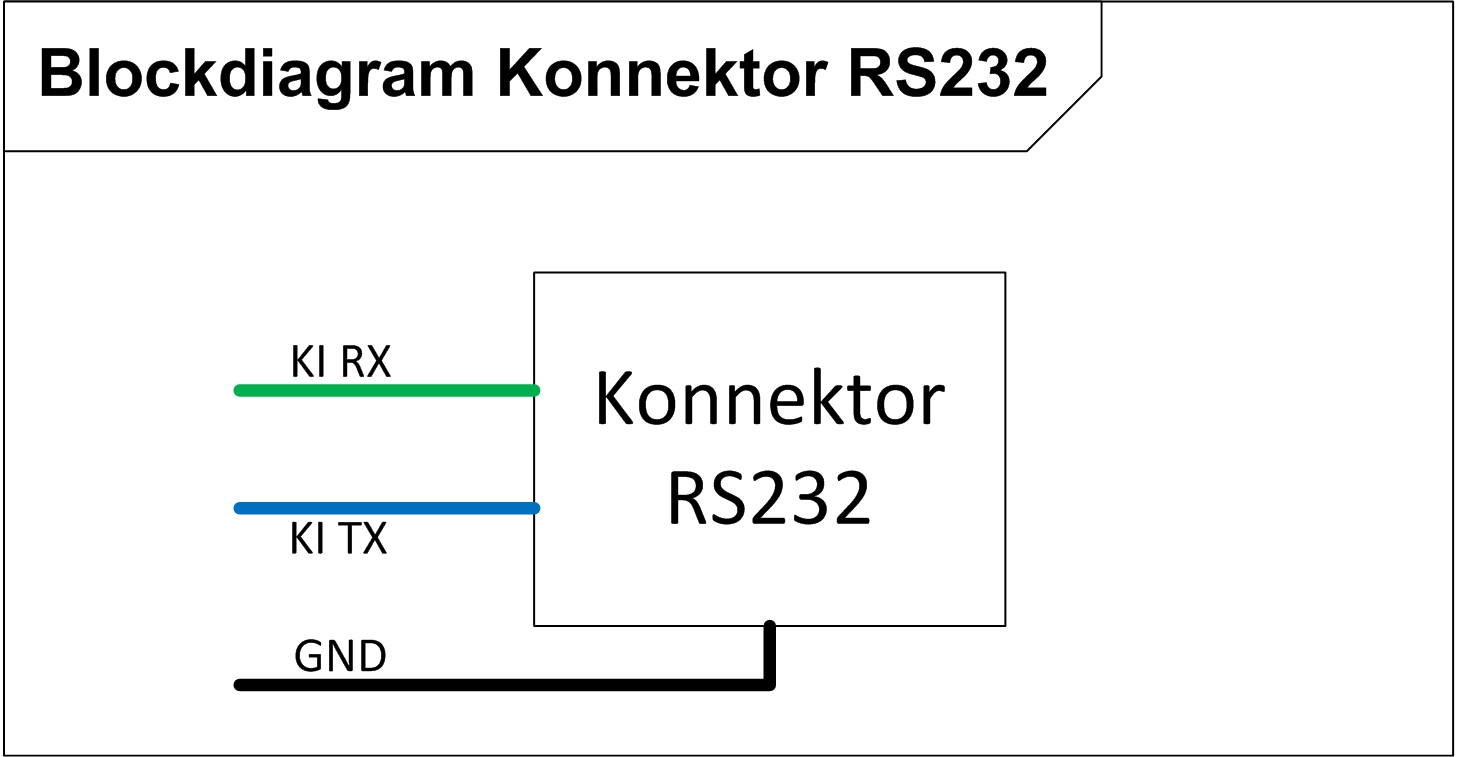
\includegraphics[scale=1]{billeder/konnektor_rs232}
\caption{Blokdiagram for konnektor RS232}
\label{fig:KonnektorRS232}
\end{figure}
\subsubsection{Signalbeskrivelser:}
For signalbeskrivelser se \textit{tabel~\ref{table:konnektorRS232}}
\begin{table}[H]
\begin{tabular}{|p{3cm}|p{3cm}|p{3cm}|p{4.5cm}|} \hline
\cellcolor[gray]{0.85}Signal navn& \cellcolor[gray]{0.85}Type &\cellcolor[gray]{0.85}Spænding&\cellcolor[gray]{0.85}Beskrivelse\\ \hline
KI RX & Analog & $\pm$13V & RX forbindes til DB9 stikket, som føres via kabel til KI modulet.\\ \hline
KI TX & Analog & $\pm$25V & TX forbindes til DB9 stikket, som føres via kabel til KI modulet. \\ \hline
GND & Ground & 0V & Ground i systemet \\ \hline
\end{tabular}
\caption{Tabel over signaler i konnektor RS232 blokken}
\label{table:konnektorRS232}
\end{table}
\subsection{DC - DC PowerSupply 5V}
Se powersuply afsnittet.
\newpage
\section{Opbygning af design}
Nedenfor følger opbygningen af designet for de forskellige blokke i UART blokken. Dette vil blive beskrevet med Multisim designs, samt udregninger. 
\subsection{SM UART}
Designet af denne blok er beskrevet i SM, under design af PSoC UART
\subsection{Indikator TX og Indikator RX}
Da de to blokke næsten designes ens, beskirves de i samme design. \\
Indikator TX og RX skal vise om der sendes eller modtages data. Dette gøres med to dioder der sidder fra 5V ned til RX og TX.
\begin{figure}[H]
\centering
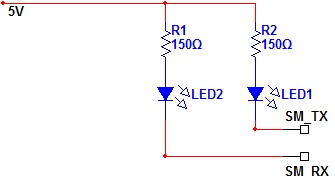
\includegraphics[scale=1]{billeder/Indikator_RX_TX}
\caption{Realisering af Indikator TX og RX}
\label{fig:Indikator_RX_TX}
\end{figure}
\subsubsection{Beregning}
Beregning af modstandværdi.\\
Diodedata fra datablad:\\
Grøn LED: V\_LED1 = 2V, I\_LED1 = 20mA\\
Gul LED: V\_LED2 = 2.1V, I\_LED2 = 20mA\\
R1 = (5V - 2.1V) / 20mA = 145 ohm \\
Nærmest standardværdi: 150 ohm, der vælges en modstand på \textbf{150 ohm} \\
R2 = (5V - 2V) / 20mA = 150 ohm \\
Standardværdi: 150 ohm, der vælges en modstand på \textbf{150 ohm} \\
\newpage
\subsection{Level konverter}
Level konverter er bygget op omkring st3232cn som konvertere TTL / CMOS signaler om til RS232 protokol signaler.
Designet er taget fra databladets APPLICATION CIRCUITS. (footnote) 
\begin{figure}[H]
\centering
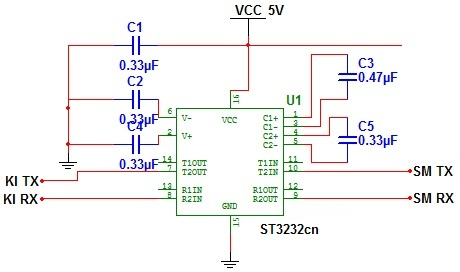
\includegraphics[scale=1]{billeder/Level_konvertor_dia}
\caption{Realisering af level konverter blok}
\label{fig:Lvl_konverter}
\end{figure}
De enkel kondensator værdier er også taget fra databladets APPLICATION CIRCUITS.(footnote) 
\subsection{Konnektor RS232}
For at forbinde RS232 kablet til SM monteres der et DB9 stik. Forbindelsen mellem SM og KI er en kablet forbindelse. I SM sidder der et DB9 stik der forbindes med kablet.
\begin{figure}[htbp] \centering
\begin{minipage}[c]{0.48\textwidth} \centering
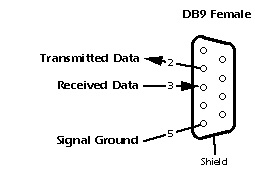
\includegraphics[scale=1]{billeder/konnektor.jpg} 
\end{minipage} \hfill
\begin{minipage}[c]{0.48\textwidth} \centering
\includegraphics[scale=1]{billeder/konnektor_dia.jpg} 
\end{minipage} \\ 
\begin{minipage}[b]{0.48\textwidth}
\caption{RS232 forbindelser på DB9} 
\label{fig:Blokdiagram_12V}
\end{minipage} \hfill
\begin{minipage}[b]{0.48\textwidth}
\caption{realisering af konnektor} 
\label{fig:Konnektor}
\end{minipage}
\end{figure}
\newpage
\subsection{Realisering af UART blok}
Samlede diagram over UART blok
\begin{figure}[H]
\centering
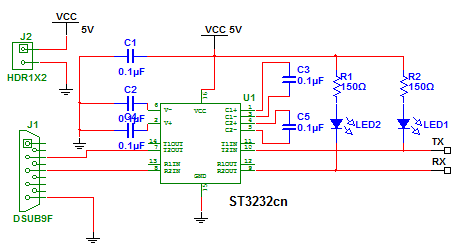
\includegraphics[scale=1]{billeder/HWUART}
\caption{Realisering for UART Blok}
\label{fig:SMHWUARTB}
\end{figure}
